\documentclass[twocolumn]{article}

%%%%%%%%%%%%%%%%%%%%%%%%%%%%%%%
% STYLES - EDIT THESE WITH CARE
%%%%%%%%%%%%%%%%%%%%%%%%%%%%%%%

% Load basic packages
\usepackage{balance}  % to better equalize the last page
\usepackage{graphics} % for EPS, load graphicx instead 
\usepackage{txfonts}
\usepackage{times}    % comment if you want LaTeX's default font
\usepackage{color}
\usepackage{textcomp}
\usepackage{booktabs}
%\usepackage{ccicons}
\usepackage{todonotes}
\usepackage{float}
\usepackage{url}  
\usepackage{titling}	% allows you to move title up the page
\usepackage[pdftex]{hyperref}

% font  sizes
\usepackage{sectsty}			% set font sizes			
\sectionfont{\Large}			% (assumes default font size 10pt)
\subsectionfont{\large}
\subsubsectionfont{\large}
\paragraphfont{\normalsize}

% positioning
\setlength{\parindent}{0em}		% remove indent for new paragraph
\setlength{\parskip}{1em}		% space above paragraph
\setlength{\columnsep}{2em}		% distance between columns
\setlength{\droptitle}{-10em}

% llt: Define a global style for URLs, rather that the default one
\makeatletter
\def\url@leostyle{%
  \@ifundefined{selectfont}{\def\UrlFont{\sf}}{\def\UrlFont{\small\bf\ttfamily}}}
\makeatother
\urlstyle{leo}

\usepackage[hyphenbreaks]{breakurl}	% make URLs within one column
\usepackage[hypens]{url}
\def\UrlBreaks{\do\/\do-}

% To make various LaTeX processors do the right thing with page size.
\def\pprw{8.27in}
\def\pprh{11.69in}
\special{papersize=\pprw,\pprh}
\setlength{\paperwidth}{\pprw}
\setlength{\paperheight}{\pprh}
\setlength{\pdfpagewidth}{\pprw}
\setlength{\pdfpageheight}{\pprh}

%%%%%%%%%%%%%%%%%%%%%%%%%%%%%%%
% END OF STYLES 
%%%%%%%%%%%%%%%%%%%%%%%%%%%%%%%

% TITLE
\title{Robot Eyes Report}
\author{David Kenny, Jamie Kerr\\BSc (Hons) Applied Computing}
\date{March 2016}



%%%%%%%%%%%%%%%%%%%%%%%%%%%
% MAIN DOCUMENT STARTS HERE
%%%%%%%%%%%%%%%%%%%%%%%%%%%

% BEGIN DOCUMENT
\begin{document}

% add title
\maketitle

%%%%%%%%%%%
%%%%%%%%%%%

\begin{abstract}

The team was given the task of creating a disparity map from a pair of stereo images using techniques that were talked about in class. 

\end{abstract}

%%%%%%%%%%%
%%%%%%%%%%%

\section{Introduction}
\vspace{-1ex}

The assignment required the team to acquire new knowledge of computer vision by producing their own disparity map from scratch using Matlab. We were encouraged to experiment with variables and publish the results of the findings. This report details the experiments that the team performed and the notable results that were acquired from them. 

%%%%%%%%%%%
%%%%%%%%%%%

\section{Background}
\vspace{-1ex}

A disparity map \cite{disparitymap} is used to show the difference between a pair of stereo images. The disparity is used to calculate depth information from a combination of the images. 

The disparity value is the value of the shift required to get the minimum sum of squared differences \cite{introssd} for that pixel or section of the image. 

Stereo pairs are images typically taken with only a slight difference in the placement of the cameras. Preferably the camera settings should be the same and the hardware should be the same as well to ensure that the images are as similar as possible.

The information gained from the disparity map will be useful to robots and machinery to provide extra depth information to base movements or actions on for example google car \cite{googlecar}.  

%%%%%%%%%%%
%%%%%%%%%%%
\section{Description of Algorithm}
\vspace{-1ex}

The team used a brute force method to gain their results using this method meant that the run time was extremely high due the fact of a disparity value having to be calculated for every pixel of the image with no shortcuts. 

This was a problem when the team were testing their program. Also since we were learning at the same time it didn't help as a simple error could take in excess of 10 minutes to produce a result even on a 100 x 100 image which lowered the teams productivity. 

%TODO:Add another potential algorithms.

The team discovered an algorithm called ENCC \cite{ENCC} which produces an estimate of disparity with sub pixel accuracy. This could have been used in place of the brute force method to create a disparity map but may not have had the same accuracy. 

%%%%%%%%%%%
%%%%%%%%%%%
\section{Description of Images Used}
\vspace{-1ex}

The team used the stereo images provided on the VLE to create their program. The pair that was mainly used was the bookcase image shown in figure \ref{fig:testR}. It was selected as there are clear levels of depth between the different books and the team thought that they would produce a noteworthy result. 

\begin{figure}[H]
\centering
  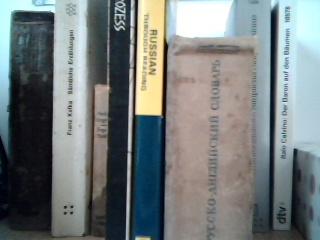
\includegraphics[width=40mm]{Figures/testR}
    \caption{Bookcase}~\label{fig:testR}
\end{figure} 

The other pair that the team used was the "Scene" pair which we had seen used a lot in the computer vision community \cite{sceneusage} \cite{sceneusage2} for various benchmark tests including disparity maps. We believe that this is due to there being an obvious deviation of layers in the image. The image also has a small resolution too which means that it won't take long to produce a result.  

\begin{figure}[H]
\centering
  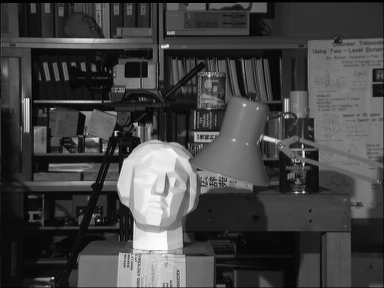
\includegraphics[width=40mm]{Figures/scene}
    \caption{Scene}~\label{fig:scene}
\end{figure} 

We used our own image which was taken with an iPhone 6S. It has an iPad box in the background and a bottle of coke in front of it to indicate clear layers of depth in the stereo pair.

\begin{figure}[H]
\centering
  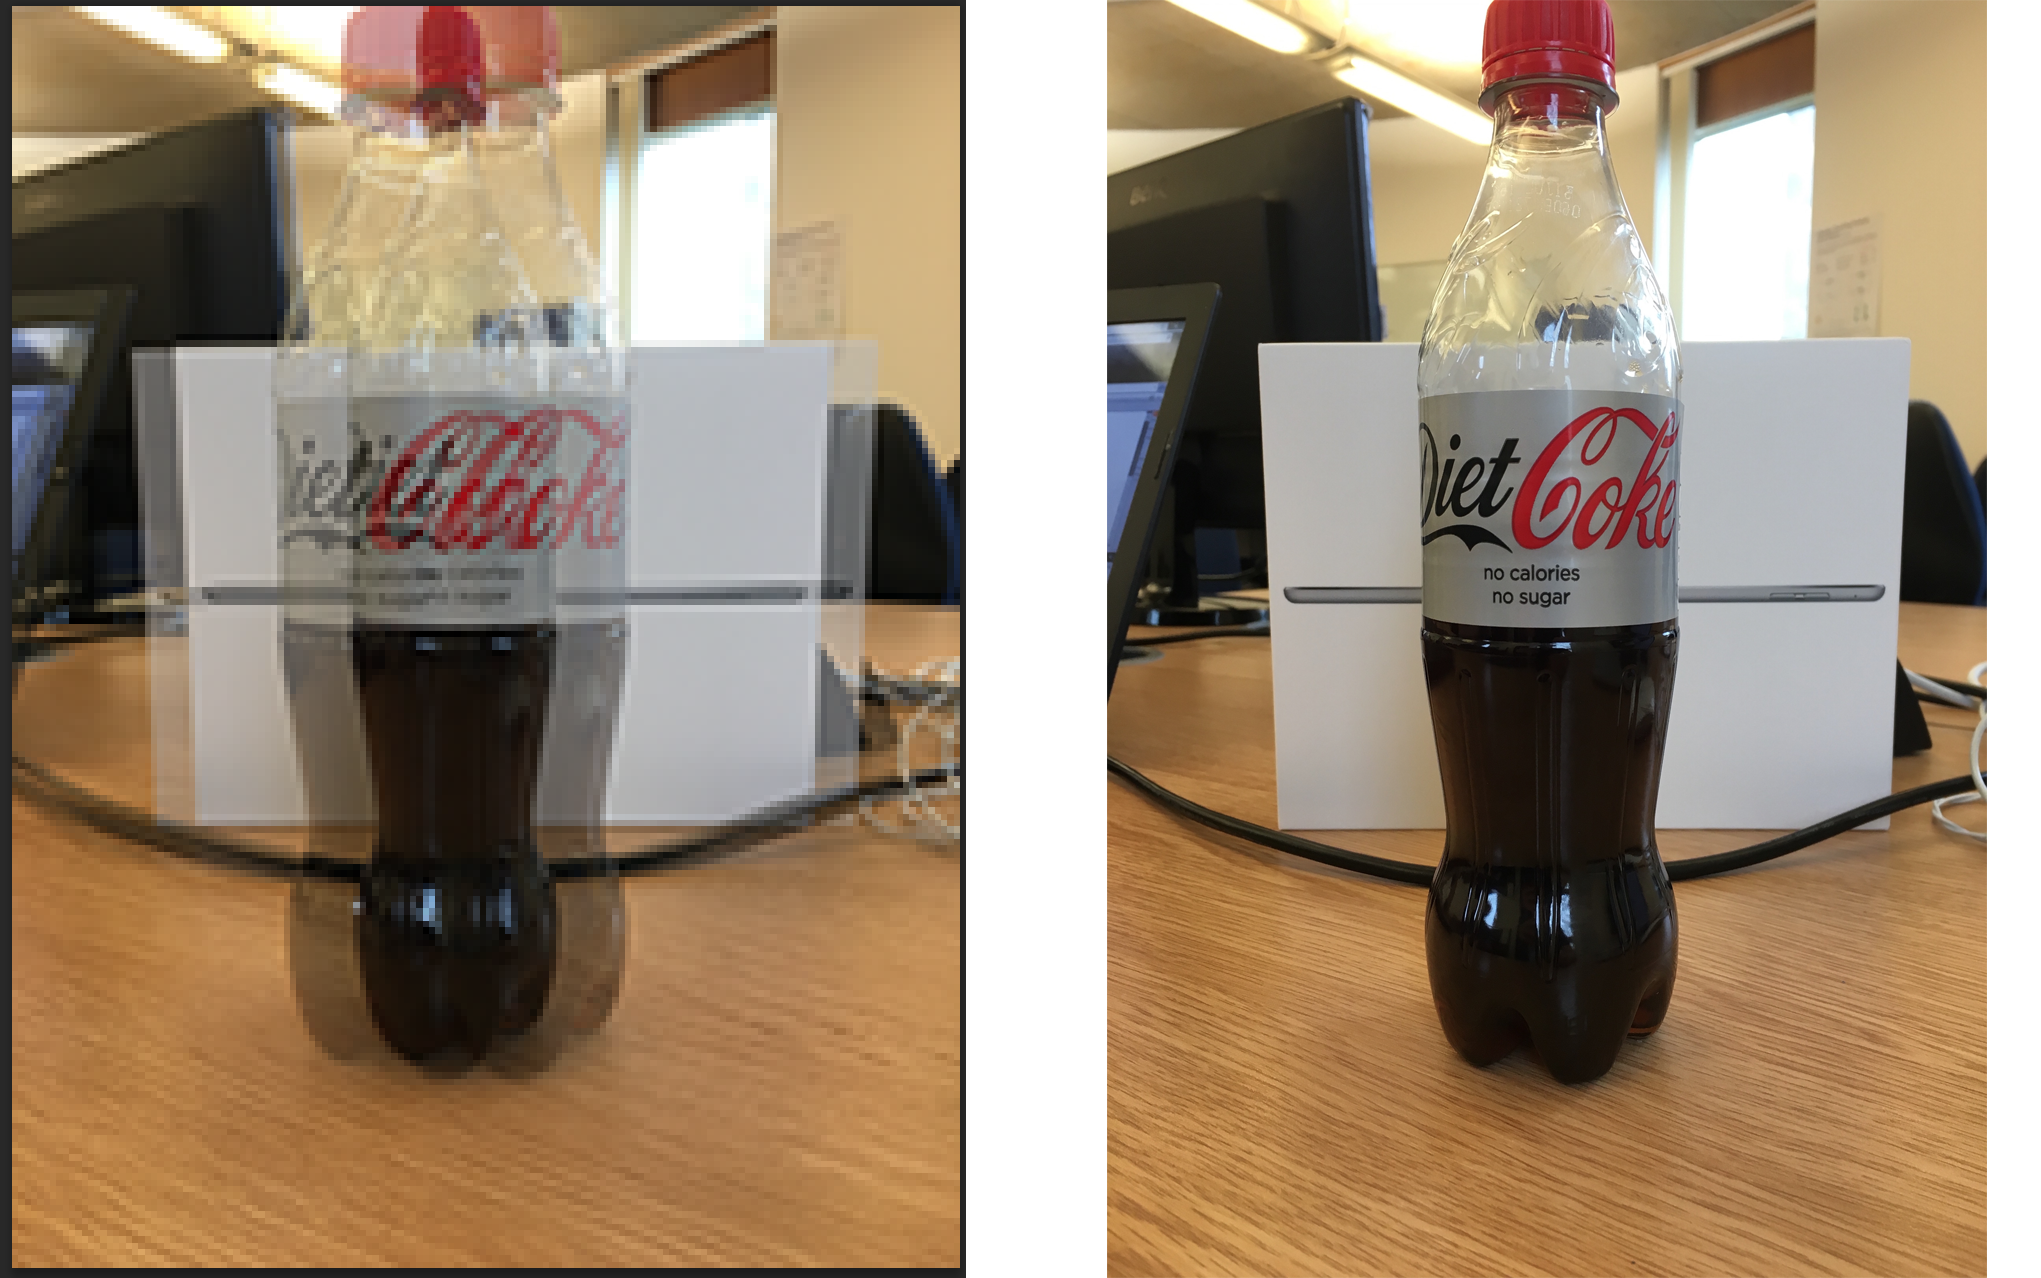
\includegraphics[height=30mm]{Figures/Coke_Image}
    \caption{Our Image}~\label{fig:CokeScene}
\end{figure} 

The image was scaled down from a resolution of 3024 x 4032 to 150 x 200 using photoshop for testing purposes as it would take significantly less time to compute. On the left of figure \ref{fig:CokeScene} is the left and the right images overlaid. When the images were taken the team used a table to place the camera on to ensure that the position of the camera remained constant from taking the left and right image. We were aware that rotation of the camera wasn't fixed which can result in a sub optimal stereo pair.  

%Example images + stereo pair that was taken in the labs. 

%%%%%%%%%%%
%%%%%%%%%%%

\section{Results}
\vspace{-1ex}

The team created a program that worked out the disparity and outputted the SSD(Sum of square differences) and disparity for one specific pixel. First of all we started using a search window of 15 x 15 and a support window of 3 x 3. After this was done we then started trying to create a disparity map using the SSD values for each pixel.  

The team found that the SSD values were not correctly working since it was either producing a value of 0 or 255 as the final output this was confirmed when the disparity maps pixels were either black or white. 

 We found that the displacement values had to be converted into an 8 bit unsigned integer to be correctly displayed as a greyscale image. This then resulted in figure \ref{fig:Third_Result} being produced which was a step in the right direction. 

It was noted that the black band shown in figure \ref{fig:Third_Result} is due to the padding that was added to image.  

\begin{figure}
\centering
  
\includegraphics[height=20mm]{Figures/Third_Result}
    \caption{Greyscale Output}~\label{fig:Third_Result}
\end{figure} 

After figure \ref{fig:Third_Result} was produced the team then ran a test using a 200 x 200 image. This test took over two hours to run on a modern laptop and the end result wasn't what the team were hoping to produce. This turned out to be a huge waste of productivity.  
 
\begin{figure}[H]
\centering
  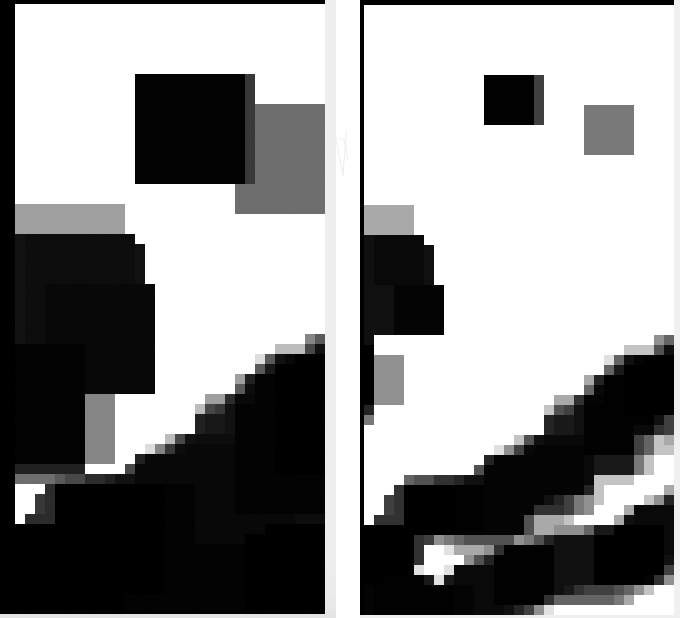
\includegraphics[height=30mm]{Figures/Search_Window_Comparison}
    \caption{Search Window}~\label{fig:Search_Window}
\end{figure} 
%We found that the images that we had been using when doing the resize down to 20 
Since the team couldn't find out much information from the corner of the books we decided to try using the scene image (figure \ref{fig:scene}) and focus on the section of the image where the lamp is in front of the head. The result that was produced from this was the image on the left of figure \ref{fig:Search_Window}. The team were pleased with this result as there was a larger variation in values. 

The result seemed pixelated the team believed that this was because of the search window size since we knew that decreasing the size of the window would increase the resolution and provide more clarity in the disparity map how ever the trade off is that noise isn't handled as much. 

The window size was reduced from 15 to 9 and the image on the right of figure \ref{fig:Search_Window} was produced. This seemed to be hopeful.

\begin{figure}[H]
\centering
  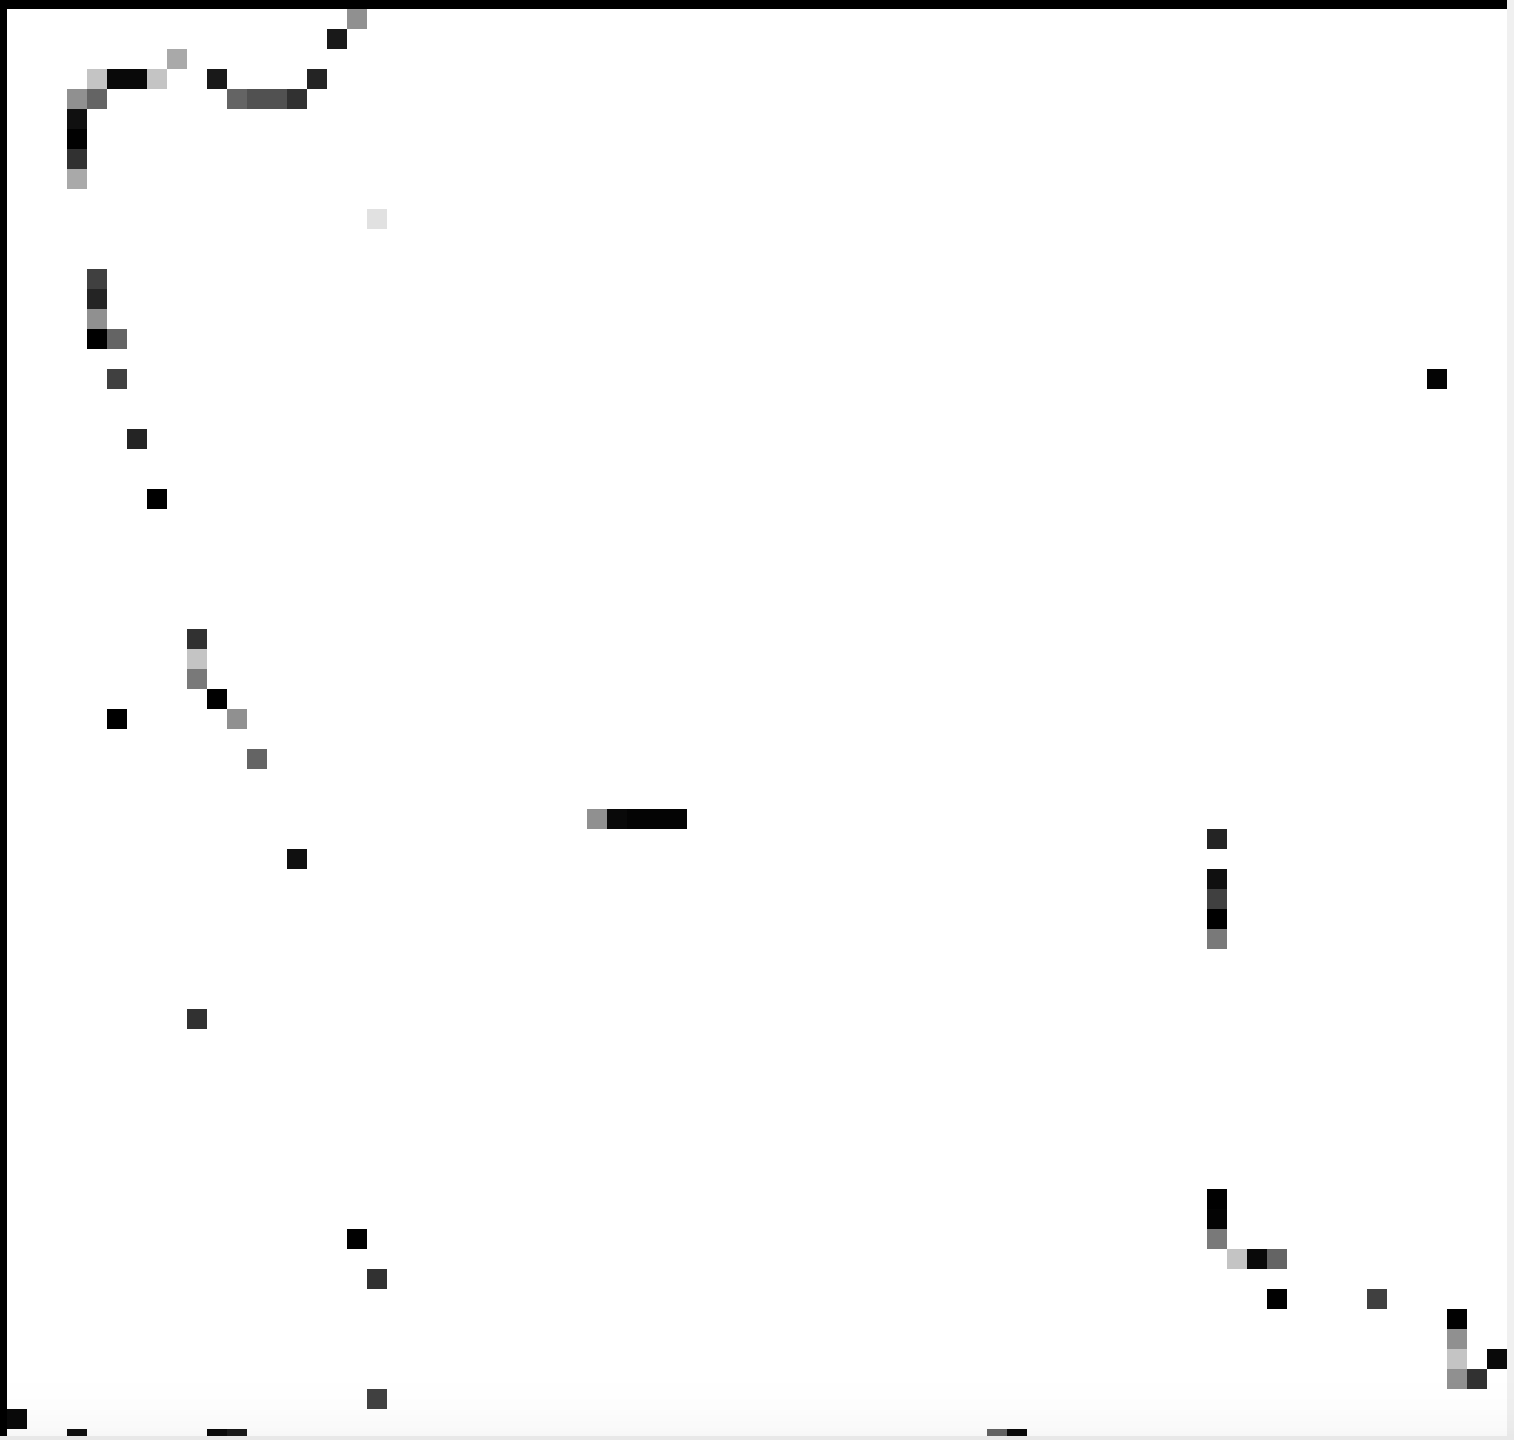
\includegraphics[height=20mm]{Figures/Coke_Result}
    \caption{Coke Result}~\label{fig:Coke_Result}
\end{figure} 

After the result in figure \ref{fig:Coke_Result} was produced on our full sized image (figure \ref{fig:CokeScene}). The team realised that the disparity map wasn't functioning correctly. Assistance was then provided by Andrew Mcneil and it was pointed out that we were using the SSD values to create the map and not the disparity values which was an oversight.  

 \begin{figure}[H]
\centering
  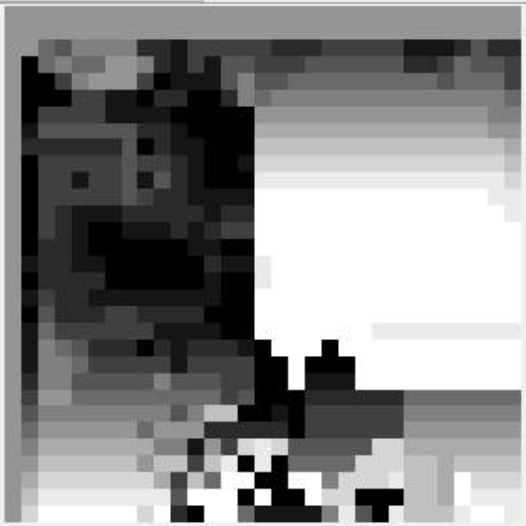
\includegraphics[height=30mm]{Figures/Disp_Vectors_1}
    \caption{Disparity vectors result}~\label{fig:Disp_Vectors_1}
\end{figure} 

After making alterations to our program to use the disparity values we managed to produce figure \ref{fig:Disp_Vectors_1}. This was produced by mapping the disparity values to a relevant greyscale value for each pixel. 

We knew that this still wasn't what we were expecting and since the structure of our program was increasingly complex it became difficult to debug. At this point the team decided to go back to the drawing board by getting rid of two weeks worth of work to when we simply had the disparity vector of one pixel being computed since the code was a lot more manageable at this point. 

We then modified the code to calculate every pixel similar to what it was doing before hand and started to get some noteworthy results instead of hardcoding values we set up variables for search window size, support window size, map height, map width and the type of algorithm.

A GUI was created during the run time of generating the maps to help run future tests this was built to increase our productivity during run time and also assist with testing. 

One problem we realised that we had created was before we were looping through the whole right image and not just the search window which was the reason why our program was taking so long. The padding was also removed as it was causing major problems when creating the maps.  

The option for the SAD matching algorithm was added in to our program as well so we could run tests to compare them. 

 \begin{figure}[H]
\centering
  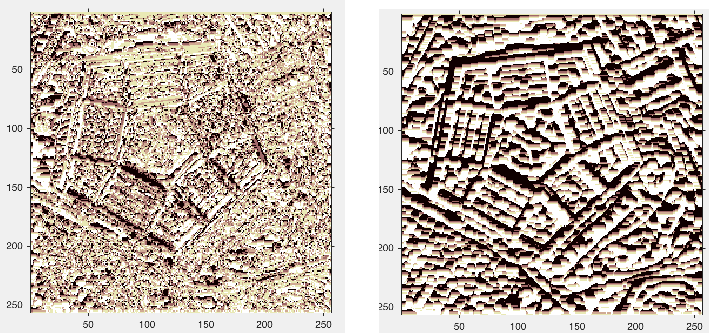
\includegraphics[height=35mm]{Figures/SSDvsSAD}
    \caption{SSD vs SAD}~\label{fig:SSDvsSAD}
\end{figure} 

Figure \ref{fig:SSDvsSAD} shows the difference between using SSD and SAD on the pentagon image. The disparity maps colours were mapped using the pink colormap function as well to produce a clearer visualisation. In this situation we believe that SAD produced a more accurate representation of depth in the image. 


 

\section{Conclusion}
\vspace{-1ex}

From the results gained, Even though they may not be exactly spot on the team felt they were on the right lines.

The team had never worked with Matlab before and were pleased with what they were able to achieve within this short space of time. 
 
The GUI that was produced helped a lot with testing and the team were pleased to have created it with no prior experience.   

The full source code for the teams work can be found in a git hub repository \cite{githublink}.

\section{Future Work} 
\vspace{-1ex}

If the team had more time available we would like to have been able to perform research on 3D imaging techniques and work on ways of optimising the matching algorithm to minimise computation. 

%%%%%%%%%%%
%%%%%%%%%%%

\section*{Acknowledgements}
The team would like to thank Andrew McNeil for his support throughout this module.

%%%%%%%%%%%
%%%%%%%%%%%

\bibliographystyle{SIGCHI-Reference-Format}
\bibliography{RobotEyes}

% END DOCUMENT
\end{document}
